\documentclass{beamer}
\setbeamertemplate{caption}[numbered]
\usepackage{graphicx}
\usepackage[utf8]{inputenc}
\usepackage[english]{babel}
\graphicspath{{Images/}}
\usepackage{comment}
\usepackage{verbatim}
\usepackage{hyperref}
\mode<presentation>
{
	\usetheme{AnnArbor}
	\usecolortheme{crane}
}

\title[Introduction to Stata]{Introduction to Stata}
\subtitle[ISRC Workshop]{Iowa Social Research Center (ISRC) Workshop}
\author[Wallace]{Desmond D. Wallace}
\institute[University of Iowa]{Department of Political Science\\The University of Iowa\\Iowa City, IA}

\date{September 15, 2017}

\begin{document}
	
\begin{frame}
	\titlepage
\end{frame}

\section{Stata Interface}
\subsection{Main Window}

\begin{frame}
	\frametitle{PC}
		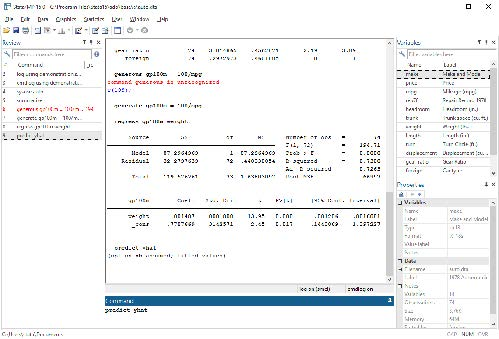
\includegraphics[scale=0.75]{main_window_pc}
\end{frame}

\begin{frame}
	\frametitle{MAC}
		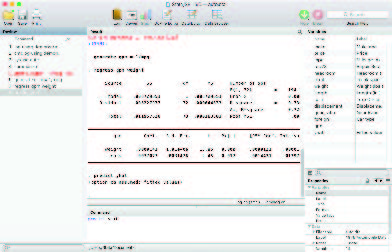
\includegraphics[scale=0.75]{main_window_mac}
\end{frame}

\begin{frame}
	\frametitle{Descriptions}
		\begin{enumerate}
			\item Command -- Type commands
			\item Results -- Executed commands and resulting output
			\begin{enumerate}
				\item Current and Command log status
			\end{enumerate}
			\item Review -- Past commands from current session
			\item Variables -- Variable list of current dataset
			\item Properties -- Displays dataset and variable properties
		\end{enumerate}
		Note: Grey Bar at Bottom of the Screen -- Displays current working directory
\end{frame}

\subsection{Toolbar}

\begin{frame}
	\frametitle{PC and MAC}
		PC: 
\includegraphics[scale=0.75]{toolbar_pc} \\
		MAC: 
\includegraphics[scale=0.25]{toolbar_mac}
\end{frame}

\begin{frame}
	\frametitle{Descriptions}
		\begin{itemize}
			\item Open -- Open a Stata-related file
			\item Save -- Save a Stata-related file
			\item Print -- Print output displayed in the results window
			\item Log -- Begin, close, suspend, or resume a log file
			\item Viewer -- Displays help files
			\item Graph -- Launches the graph window
		\end{itemize}
\end{frame}

\begin{frame}
	\frametitle{Descriptions}
		\begin{itemize}
			\item Do-file Editor -- Launches the Do-file editor
			\item Data Editor/Browser -- Launches the Data viewer
			\item Variables Manager -- Lists the variables in the current dataset; allows for the editing of variables
			\item More -- Display results that do not fit in the results window
			\item Break -- Stops the execution of a command
			\item Search Help -- Searches for help for Stata-written and user-written commands
		\end{itemize}
\end{frame}

\subsection{Data Browser}

\begin{frame}
	\frametitle{PC}
		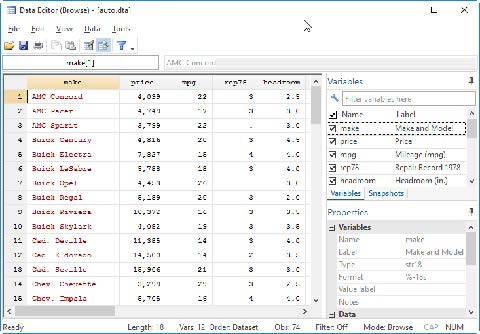
\includegraphics[scale=0.75]{data_editor_pc}
\end{frame}

\begin{frame}
	\frametitle{MAC}
		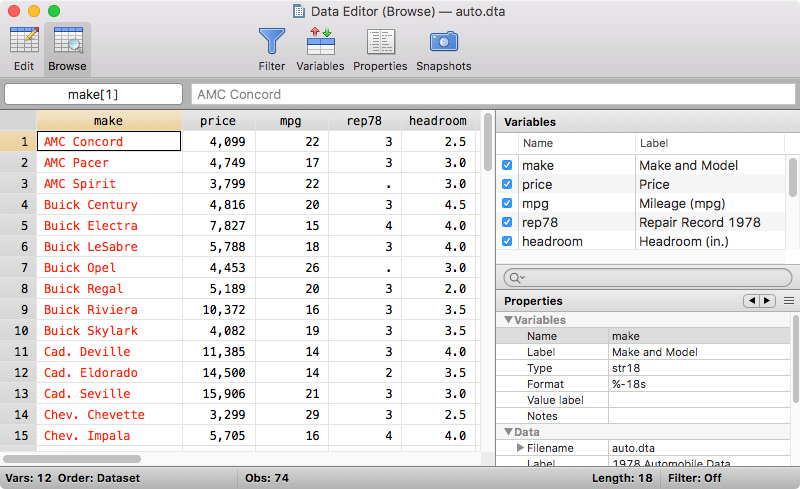
\includegraphics[scale=0.35]{data_editor_mac}
\end{frame}

\begin{frame}
	\frametitle{Modes}
		\begin{itemize}
			\item Data Editor (Edit) -- Allows one to view a dataset, and make changes
			\item Data Editor (Browse) -- Allows one to view the dataset, but not make any changes
			\item Can switch between edit mode and browse mode
			\item NOTE: When switching from browse mode to edit mode, a warning will appear, whether the user is sure about switching from browse mode to edit mode
		\end{itemize}
\end{frame}

\begin{frame}
	\frametitle{Colors}
		When viewing a dataset in the Data Editor/Browser, different types of data is represented by different colors
		\begin{itemize}
			\item Black -- Data used for various descriptive and analytic tasks
			\item Red -- Observations that contain strings, or textual data; can perform descriptive tasks, but not analytic tasks
			\item Blue -- Same as data appearing in black, except the blue represents value labels; can perform both descriptive and analytic tasks
			\item NOTE: Default is for the Data Editor/Browser to display the value labels, if any for the variables
		\end{itemize}
\end{frame}

\section{Stata Commands}
\subsection{General Command Syntax}

\begin{frame}
	\frametitle{Full Command Syntax}
		{\tiny [\textbf{by} \textit{varlist}:] \textit{command} [\textit{varlist}] [=\textit{exp}] [\textbf{if} \textit{exp}] [\textbf{in} \textit{range}] [\textit{weight}] [\textbf{using} \textit{filename}] [,\textit{options}]}
\end{frame}

\subsection{Descriptions}

\begin{frame}
	\frametitle{\textit{command}}
		\begin{itemize}
			\item Only required element of command statement
			\item Case-sensitive
			\item Commands can be abbreviated
			\item Example: To display summary statistics of a variable, or variables:
			\begin{itemize}
				\item \texttt{\underline{sum}merize}
				\item \texttt{sum}
				\item The underlined portion of \texttt{summerize} represents the abbreviation
			\end{itemize}
		\end{itemize}
\end{frame}

\begin{frame}
	\frametitle{\textit{varlist}}
		\begin{itemize}
			\item Represents one variable, or at least two variables
			\item Case-sensitive
			\item Variables can be abbreviated to minimum number of letters that makes variable unique
			\item To refer to several variables at the same time:
				\begin{itemize}
					\item Use the * symbol
					\item Use a name range
				\end{itemize}
		\end{itemize}
\end{frame}

\begin{frame}
	\frametitle{\textit{=exp}}
		\begin{itemize}
			\item Used to generate new variables
			\item Can include variables in expression statements
			\item Usually an arithmetic expression
				\begin{itemize}
					\item Can include the four basic operation symbols ($+$, $-$, $*$, $/$)
					\item Can use \^{} for an exponentiation statement
					\item Can include other functions, such as $abs$ and $log$
					\item Can include parentheses to manage order of operations
				\end{itemize}
		\end{itemize}
\end{frame}

\begin{frame}
	\frametitle{if \textit{exp} and in \textit{range}}
		\begin{itemize}
			\item Used to restrict dataset to a subsample of interest
			\item Represented as a logical statement that is either true or false
			\item Relation operators are $<$, $<=$, $==$, $>=$, $>$, and $!=$
			\item Can also specify a range of observations
			\item Example: \texttt{in 1/10} refers to the first ten observations of a dataset
		\end{itemize}
\end{frame}

\begin{frame}
	\frametitle{\textit{weights}}
		\begin{itemize}
			\item Used to weigh the observations
			\item Example: survey data typically uses weights in order to make the sample representative of the population
			\item Used in conjunction with many commands
		\end{itemize}
\end{frame}

\begin{frame}
	\frametitle{using \textit{filename}}
		\begin{itemize}
			\item Introduces a file into the command
			\item File can be on the computer, on a network, or on the internet
		\end{itemize}
\end{frame}

\begin{frame}
	\frametitle{\textit{options}}
		\begin{itemize}
			\item Most commands have additional options that the user can specify
			\item Look at the help file for the command to list its options
		\end{itemize}
\end{frame}

\begin{frame}
	\frametitle{by \textit{varlist}}
		\begin{itemize}
			\item Used to execute a command for groups of observations defined by distinct values of the variable(s) specified
			\item Command in question has to be "byable"
			\item Data must be sorted by the grouping variable
			\item If data is not pre-sorted, use \texttt{bysort}
		\end{itemize}
\end{frame}

\section{Do-Files}

\subsection{Introduction}

\begin{frame}
	\frametitle{What are Do-files?}
		\begin{itemize}
			\item Typically, the Stata command line only allows the user to run individual commands, not collectively.
			\item A Do-file is a file that allows the user to run a number of commands at once.
			\item Do-files allow the user to keep a record of their analysis.
		\end{itemize}
\end{frame}

\subsection{Components}

\begin{frame}
	\frametitle{Commands}
		\begin{itemize}
			\item Do-files can consist of commands that require either a single line, or multiple lines.
			\item Commands that span a single line are the same as typing the command into the command line on the main Stata window.
			\item Commands that span multiple lines requires a delimiter (i.e. a character, or group of characters, Stata recognizes signifying the end of the command).
			\item The default delimiter is a carriage return (CR)
			\item Can treat carriage return as a comment using three forward slashes \texttt{///}.
			\item Commands that run multiple lines cannot be executed in the main Stata command line.
		\end{itemize}
\end{frame}

\begin{frame}
	\frametitle{Comments}
		\begin{itemize}
			\item Do-files allow the user to insert any necessary comments with respect to the Do-file.
			\item Ways to include comments:
				\begin{itemize}
					\item An asterisk -- \texttt{*}
					\item Enclosed with -- \texttt{/* */}
				\end{itemize}
			\item Lines that are commented are not executed by Stata.
		\end{itemize}
\end{frame}

\subsection{Execution}

\begin{frame}
	\frametitle{Execution}
		\begin{itemize}
		\item There are two ways to execute commands in a Do-file.
			\begin{itemize}
				\item Method 1: Execute the entire file.
				\item Method 2: Execute the file in pieces via highlighting the specific code you want to execute.
			\end{itemize}
		\item You can also nest Do-files within other Do-files.
		\end{itemize}
\end{frame}

\begin{frame}
	\frametitle{Commands}
	\begin{itemize}
		\item \texttt{\underline{doed}it} launches the Do-file editor with a blank do-file.
		\item \texttt{\underline{doed}it [\textit{filename}]} launches the Do-file editor with the specified do-file.
		\item \texttt{do \textit{filename}} executes all commands stored in specified do-file. 
	\end{itemize}
\end{frame}

\section{Basic Commands}
\subsection{Opening Data}

\begin{frame}
	\frametitle{Opening the Data}
		\begin{itemize}
			\item The command for opening a dataset in Stata is \texttt{use}.
			\item If a dataset is already open, opening a new dataset requires including the option \texttt{clear} with the \texttt{use} command.
			\item Examples
				\begin{itemize}
					\item Example: \texttt{use \textit{filename}} works if there is no data in Stata's memory.
					\item Example: \texttt{use \textit{filename}, clear} works if data is already in memory.
				\end{itemize}
		\end{itemize}
\end{frame}

\subsection{Data Inspection}

\begin{frame}
	\frametitle{\texttt{describe}}
		\texttt{\underline{d}escribe} provides basic information about a Stata dataset. \\
		\texttt{\underline{d}escribe [\textit{varlist}]} provides basic information about specified variables.
			\begin{itemize}
			\item Number of observations and variables
			\item Size of file (in bytes)
			\item Most recent timestamp
			\item Summary Information
				\begin{itemize}
					\item Variable Name
					\item Storage Type
					\item Display Format
					\item Value Label
					\item Variable Label
				\end{itemize}
			\end{itemize}
\end{frame}

\begin{frame}
	\frametitle{\texttt{summarize}} 
		\texttt{\underline{sum}marize} gives summary statistics for the variables in the dataset. \\
		\texttt{\underline{sum}marize [\textit{varlist}]} provides summary statistics for specified variables.
			\begin{itemize}
				\item Number of Observations
				\item Mean
				\item Standard Deviation
				\item Minimum
				\item Maximum
			\end{itemize}
		The option \texttt{detail} provides additional statistics.
			\begin{itemize}
				\item Skewness
				\item Kurtosis
				\item Four largest (smallest) values
				\item Various percentiles (1, 5, 10, 25, 50, 75, 90, 95, 99)
			\end{itemize}
\end{frame}

\begin{frame}
	\frametitle{\texttt{tabulate} (One-way)}
		\begin{itemize}
			\item \texttt{\underline{tab}ulate \textit{varname}} or \texttt{tab1 \textit{varlist}} produces a frequency table for a variable, or list of variables.
				\begin{itemize}
					\item Example: \texttt{tab \textit{var1}}
				\end{itemize}
			\item However, using \texttt{tab} alone will not provide frequencies with respect to missing observations.
			\item Frequencies of missing observations requires including the option \texttt{\underline{m}issing}.
				\begin{itemize}
					\item Example: \texttt{tab \textit{var1}, m}
				\end{itemize}
			\item Default is to produce a frequency table featuring value labels
			\item Creating a frequency table without value labels requires including the option \texttt{\underline{nol}abel}
				\begin{itemize}
					\item Example: \texttt{tab1 \textit{var1 var2 var3}, nol}
				\end{itemize}
		\end{itemize}
\end{frame}

\begin{frame}
	\frametitle{\texttt{tabulate} (Two-way)}
		\begin{itemize}
			\item \texttt{\underline{tab}ulate \textit{varname1} \textit{varname2}} or \texttt{tab2 \textit{varlist}} produces a contingency table for a pair of variables.
				\begin{itemize}
					\item Example: \texttt{tab \textit{var1} \textit{var2}}
					\item Usually, dependent variable is listed first, followed by independent variable
				\end{itemize}
			\item Can report row, column, and cell relative frequencies using \texttt{\underline{r}ow}, \texttt{\underline{co}lumn}, and \texttt{\underline{ce}ll} options.
			\item Can report various measures of association (e.g., Chi-Squared ($\chi^2$), Cramer's V) (See \texttt{help tabulate twoway} for full list of options)
		\end{itemize}
\end{frame}

\begin{frame}
	\frametitle{\texttt{codebook}}
		\texttt{codebook} examines the variable names, labels, and data to produce a codebook describing the dataset. \\
		\texttt{codebook [\textit{varlist}]} provides a codebook for the specified variables.
			\begin{itemize}
				\item Variable Name and Variable Label
				\item Type
				\item Value Label
				\item Range (Smallest and Largest Values)
				\item Unique Values
				\item Units
				\item Missing
				\item Tabulation (Small number of unique values)
					\begin{itemize}
						\item Frequency
						\item Numeric Value
						\item Value Label
					\end{itemize}
			\end{itemize}
\end{frame}

\section{Resources}
\subsection{Features}

\begin{frame}
	\frametitle{New Features in Stata 15}
		Stata 15 includes a number of refinements and new features, including:
			\begin{itemize}
				\item \texttt{bayes:} prefix for estimating Bayesian regression models \\(Example: \texttt{bayes:~regress \textit{depvar} \textit{indvar1} \textit{indvar2}})
				\item Markdown and dynamic documents -- Integrating Stata code into documents (e.g., results graphs)
				\item Including transparency features into graphs
				\item Number of new methods
					\begin{itemize}
						\item Spatial Autoregressive Models
						\item Bayesian Multilevel Models
						\item Nonlinear Multilevel Models
					\end{itemize}
			\end{itemize}
		\href{https://www.stata.com/new-in-stata/}{Click here} for the full list of new features.
\end{frame}

\subsection{Resources}

\begin{frame}
	\frametitle{Available Resources}
		\begin{itemize}
			\item \href{http://www.stata-press.com/manuals/documentation-set/}{Stata Documentation}
			\item \href{http://www.stata-press.com/}{Stata Press}
			\item \href{https://stats.idre.ucla.edu/stata/}{UCLA Institute for Digital Research and Education}
			\item \href{http://www.stata.com/contactadmin/link.php?M=6471092&N=1178&L=1430&F=H}{Stata Cheat Sheets}
			\item \href{http://ppc.uiowa.edu/isrc/workshops}{ISRC Workshops}
		\end{itemize}
\end{frame}

\begin{frame}
	\begin{center}
		\begin{LARGE}
			Any Questions?
		\end{LARGE}
	\end{center}
\end{frame}

\end{document}
